% --------------------------------------------------------------
% This is all preamble stuff that you don't have to worry about.
% Head down to where it says "Start here"
% --------------------------------------------------------------
 
\documentclass[12pt]{article}
 
%Russian-specific packages
%--------------------------------------
\usepackage[T2A]{fontenc}
\usepackage[utf8]{inputenc}
\usepackage[russian]{babel}
%--------------------------------------
 
\usepackage[margin=1in]{geometry}
\usepackage{amsmath,amsthm,amssymb}
\usepackage{verbatim}

%--------------------------------------
\usepackage{graphicx}%Вставка картинок правильная
\usepackage{float}%"Плавающие" картинки
\usepackage{wrapfig}%Обтекание фигур (таблиц, картинок и прочего)
\graphicspath{{images/}}
\DeclareGraphicsExtensions{.pdf,.png,.jpg}
%--------------------------------------
 

\newcommand{\N}{\mathbb{N}}
\newcommand{\Z}{\mathbb{Z}}
\newcommand{\R}{\mathbb{R}}
 
\newenvironment{theorem}[2][Теорема]{\begin{trivlist}
\item[\hskip \labelsep {\bfseries #1}\hskip \labelsep {\bfseries #2.}]}{\end{trivlist}}
\newenvironment{lemma}[2][Лемма]{\begin{trivlist}
\item[\hskip \labelsep {\bfseries #1}\hskip \labelsep {\bfseries #2.}]}{\end{trivlist}}
\newenvironment{exercise}[2][Упражнение]{\begin{trivlist}
\item[\hskip \labelsep {\bfseries #1}\hskip \labelsep {\bfseries #2.}]}{\end{trivlist}}
\newenvironment{problem}[2][Задача]{\begin{trivlist}
\item[\hskip \labelsep {\bfseries #1}\hskip \labelsep {\bfseries #2.}]}{\end{trivlist}}
\newenvironment{statement}[2][Утв.]{\begin{trivlist}
\item[\hskip \labelsep {\bfseries #1}\hskip \labelsep {\bfseries #2.}]}{\end{trivlist}}
\newenvironment{corollary}[2][Следствие]{\begin{trivlist}
\item[\hskip \labelsep {\bfseries #1}\hskip \labelsep {\bfseries #2.}]}{\end{trivlist}}
 
\newenvironment{solution}{\begin{proof}[Решение]}{\end{proof}}
 
\begin{document}
 
% --------------------------------------------------------------
%                         Start here
% --------------------------------------------------------------
 
\title{Домашняя работа №3}
\author{Шишацкий Михаил, 932}
\date{08.04.2020}
 
\maketitle

\begin{problem}{1}
    Сольём два дерева $T_1$ и $T_2$, для которых известно, что все ключи
     $T_1$ меньше ключей $T_2$. Без ограничения общности будем считать, что  
     $H(T_1) \geq H(T_2)$.\\

     Найдём в $T_2$ самую левую вершину (назовём её $w$) и удалим её из дерева.
     Затем в $T_1$ будем идти в правое поддерево до тех пор, пока не встретим 
     поддерево $S$, высота которого равна высоте $T_2$ после удаления вершины $w$.
     Такое поддерево найдется, т.к. изначально $H(T_1) \geq H(T_2)$, а при каждом
     спуске высота поддерева уменьшается на  $1$. \\

     \begin{figure}[H]
         \centering
         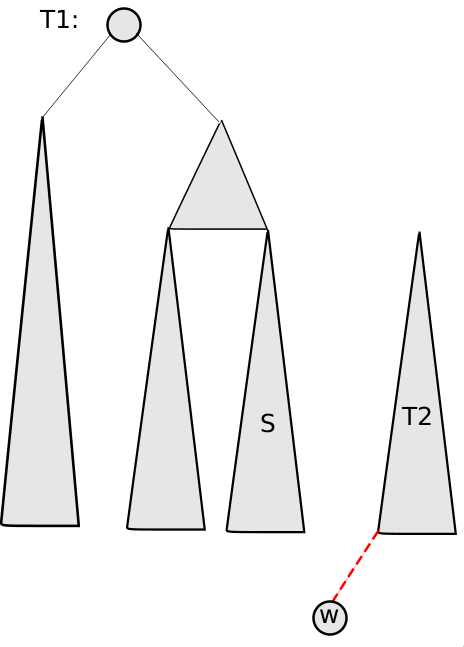
\includegraphics[width=0.4\linewidth]{Problem1_before.png}
         \caption{Подготовительные действия}
     \end{figure}

     Теперь дерево $T_1$ можно перестроить следующим образом:\\

     \begin{figure}[H]
         \centering
         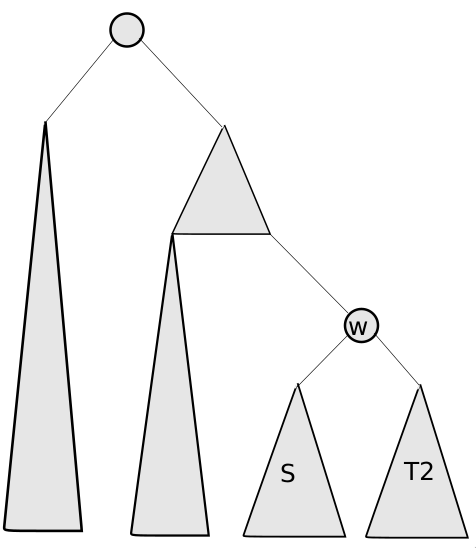
\includegraphics[width=0.4\linewidth]{Problem1_after.png}
         \caption{Слитые деревья}
     \end{figure}

     После такого перестроения ключи распорагаются в правильном порядке,
     однако мог нарушиться баланс для некоторых поддеревьев. 
     Деревья $S$ и $T_2$ сбалансированы и имеют равные высоты.
     Значит дерево с корнем $w$ тоже сбалансировано. Следовательно, мог
     нарушиться только баланс в вышестоящих вершинах из-за увеличения высоты
     правого поддерева на $1$. Значит, необходимо пройтись от $w$ к корню, 
     балансируя соответствующие вершины.\\

     Асимптотика полученного алгоритма - $O(log(max(|T_1|, |T_2|)))$. 

\end{problem}


\begin{problem}{4a}
    Для нахождения ключа, следующего за $x$, можно не хранить никакой 
    дополнительной информации в вершинах, но асимптотика такого поиска -
    $O(log(N))$ в среднем.

    Если $x$ имеет правого сына, достаточно найти в нём самый левый элемент,
    спускаясь вниз по поддереву. Найденная вершина  будет содержать искомый ключ.

    Если у $x$ нет правого сына. нужно вызвать операцию split по ключу $x$ и в 
    дереве, ключи которого больше $x$ найти самый левый элемент. Затем конечно
    же нужно обратно слить деревья операцией merge.
\end{problem}

\begin{problem}{4b}
    Чтобы искать последователя за $O(1)$, можно хранить в вершинах дерева
    следующую дополнительную информацию: указатель на следующий элемент в смысле
    порядка ключей, указатель на самую левую ноду, указатель на самую правую
    ноду. Если удастся поддерживать указатель на последователя, можно будет перейти
    к последователю по этому указателю.

    Так как все базовые операции реализуются с помощью merge и split, достаточно,
    чтобы эти операции поддерживали соответствующие поля в вершинах.\\
    
    \textbf{Merge:} Считается, что на вход merge поступают деревья, поля которых
    содержат корректную информацию об этих деревьях. Рассмотрим случай, когда 
    приоритет ключа второго дерева больше:

    \begin{figure}[H]
        \centering
        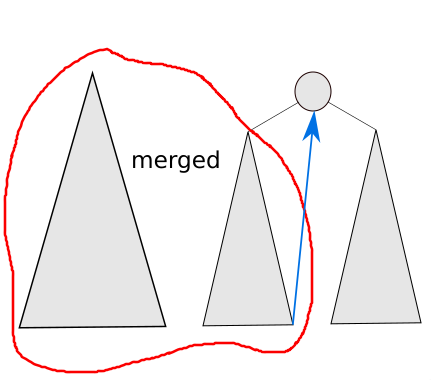
\includegraphics[width=0.4\linewidth]{Problem4_merge.png}
        \caption{merge}
    \end{figure}

    Рекурсивный вызов merge вернёт нам корректное поддерево, достаточно перейти 
    к самой правой его ноде (эта информация хранится в корне) и записать в неё
    указатель на следующий по порядку ключ, содержащийся в корне создаваемого 
    дерева. Все остальные указатели уже расставлены корректно.

    \textbf{Split:} Рассмотрим случай, когда корень текущего дерева больше, чем
    ключ, по которому производится разбиение:

    \begin{figure}[H]
        \centering
        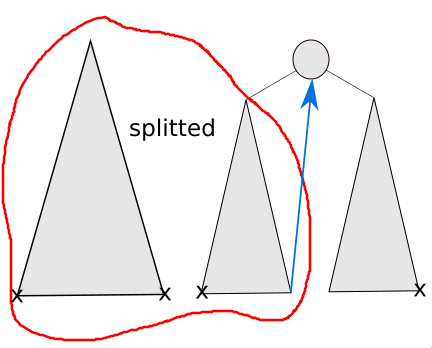
\includegraphics[width=0.4\linewidth]{Problem4_split.png}
        \caption{split}
    \end{figure}

    Рекурсивный вызов split вернёт два корректных поддерева. Необходимо записать 
    в самую правую ноду поддерева, которое мы собираемся подвесить к корню, 
    указатель на корень, как на вершину с следующим по порядку ключом. В корне
    нужно заменить указатель на самую левую ноду указателем на самую левую ноду в
    подвязываемом поддереве. Все остальные поля заполнены корректно.\\

    Для остальных случаев в методах split и merge выполняются аналогичные действия,
    просто переподвязываются ноды с других сторон.

\end{problem}

%
%\begin{problem}{5}
%    
%    Чтобы найти простой путь с максимальной суммой, можно запустить DFS из корня,
%    возвращающий структуру, хранящую максимальную сумму на простом пути, 
%    начинающемся в этой вершине и заканчивающимся где-то в поддереве, и путь,
%    соответстующий этой сумме, в виде листа. Также заведём глобальную структуру,
%    в которой в конце выполнения алгоритма будет храниться искомый путь.
%
%    \begin{verbatim}
%        int DFS(Node* v) {
%            int left_sum = DFS(v->left);
%            int right_sum = DFS(v->right);
%
%            int max_suggestion = 
%                max(left_sum, right_sum, left_sum + right_sum);
%
%            if (max_suggestion > max_sum) {
%                max_sum = max_suggestion;
%            }
%
%            return max(left_sum, right_sum);
%        }
%    \end{verbatim}
%
%
%\end{problem}


% --------------------------------------------------------------
%     You don't have to mess with anything below this line.
% --------------------------------------------------------------
 
\end{document}
